% =====================================================================
% Byzantine-Robust, Zero-Knowledge-Verifiable Federated GNN for FDIA
% Default class: IEEEtran (conference). To switch to Springer LNCS:
%   1. Replace the \documentclass line with: \documentclass{llncs}
%   2. Replace IEEEkeywords environment with \keywords{...}
%   3. Replace IEEEtran author block with \author{...}\institute{...}
%   4. Replace \bibliographystyle{IEEEtran} with \bibliographystyle{splncs04}
% =====================================================================
\documentclass[conference]{IEEEtran}
\IEEEoverridecommandlockouts

\usepackage{cite}
\usepackage{amsmath,amssymb,amsfonts,amsthm}
\usepackage{algorithm}
\usepackage{algpseudocode}
\usepackage{graphicx}
\usepackage{textcomp}
\usepackage{xcolor}
\usepackage{booktabs}
\usepackage{multirow}
\usepackage{array}
\usepackage{tikz}
\usepackage{pgfplots}
\pgfplotsset{compat=1.18}
\usetikzlibrary{shapes,arrows.meta,positioning,fit,backgrounds,calc}
\usepackage{url}
\usepackage{hyperref}

\newtheorem{theorem}{Theorem}
\newtheorem{lemma}{Lemma}
\newtheorem{proposition}{Proposition}
\newtheorem{definition}{Definition}
\newtheorem{remark}{Remark}

\begin{document}

\title{A Byzantine-Robust, Zero-Knowledge-Verifiable Federated Graph Neural Network for False Data Injection Attack Detection in Smart Grid Distribution Systems}

\author{\IEEEauthorblockN{Saurabh B.\ Koravi}
\IEEEauthorblockA{\textit{School of Computer Engineering and Technology} \\
\textit{MIT World Peace University}\\
Pune, India \\
saurabh.koravi@mitwpu.edu.in}
\and
\IEEEauthorblockN{Reshma Sonar}
\IEEEauthorblockA{\textit{School of Computer Engineering and Technology} \\
\textit{MIT World Peace University}\\
Pune, India \\
reshma.sonar@mitwpu.edu.in}
}

\maketitle

\begin{abstract}
False data injection attacks (FDIAs) silently corrupt the state-estimation pipeline of modern smart-grid distribution systems, evading classical residual checks and degrading downstream control. Machine-learning detectors achieve high accuracy but typically demand centralized aggregation of sensitive SCADA telemetry across utilities, raising privacy, regulatory, and competitive concerns. Federated learning (FL) avoids data sharing, yet plain FedAvg admits a single Byzantine client to bias the global detector arbitrarily, and prior verifiable-FL pipelines that stack zero-knowledge ML inference proofs, trusted-execution attestation, and Byzantine-fault-tolerant consensus on the detection critical path produce end-to-end latencies that violate grid control deadlines. We propose a three-tier architecture that integrates: (i)~a Graph Attention Network~v2 (GATv2) detector that consumes the bus--branch topology of a distribution feeder as a heterogeneous graph and runs at substation edge nodes with $\approx$1.3\,ms inference; (ii)~a Byzantine-robust federated aggregator using Multi-Krum, where each client submits an $\ell_2$-norm-bounded gradient accompanied by a compact zero-knowledge range proof that $\|\Delta w\|_2 \le \tau$; and (iii)~a hash-chain audit ledger that anchors round identifiers, accepted gradient digests, and rejected client identifiers. The central design principle is to \emph{decouple} three latency paths: real-time edge detection ($\approx$1\,ms), asynchronous federated rounds (seconds), and audit anchoring (relaxed). On the IEEE 33-bus distribution feeder simulated with pandapower under unobservable FDIA attacks across 5--10 simulated utilities, the proposed system achieves an F1 score of \textbf{0.641} (averaged across two seeds) with the Multi-Krum + ZKP configuration, recovers within 0.4 F1 points of the centralized GATv2 oracle, and tolerates 40\% Byzantine clients under the unbounded-norm attack of Fang et al.~(F1=0.581) where plain FedAvg collapses to F1=0.000. The ZK gradient-bound proof rejects 100\% of Byzantine gradients in our experiments while adding only 7.5\% to the per-round upload size. Limitations including CPU-only validation, simulated grid data, and TEE attestation deferred to future work are discussed explicitly.
\end{abstract}

\begin{IEEEkeywords}
False data injection attack, federated learning, graph neural network, Byzantine robustness, zero-knowledge proof, smart grid security, distribution system.
\end{IEEEkeywords}

\section{Introduction}
The digitalization of distribution systems---driven by distributed energy resources, advanced metering infrastructure, and substation automation---has dramatically widened the cyber-physical attack surface of modern power grids~\cite{nistir7628r1,achaal2024sgsurvey}. Among the most consequential threats is the \emph{false data injection attack} (FDIA) introduced by Liu, Ning, and Reiter~\cite{liu2009false,liu2011false}: a class of stealthy attacks that craft measurement biases lying in the column space of the measurement Jacobian, thereby evading the chi-square residual test that guards classical weighted-least-squares state estimation. A decade of follow-up surveys~\cite{deng2017fdia,musleh2020survey,reda2022comprehensive,irfan2024survey} confirms that FDIAs remain unresolved in deployed grids and that data-driven detectors---convolutional, recurrent, and graph-based~\cite{he2017realtime,niu2019dynamic,mukherjee2022deep,yin2022powerfdnet,boyaci2022gnn,boyaci2022joint,takiddin2023generalized}---offer the most promising line of defense.

Three open problems remain. \textbf{First, data centralization is impractical}: SCADA, AMI, and PMU streams contain commercially and personally sensitive operational telemetry, and cross-utility sharing is restricted by NERC CIP, GDPR, and competitive concerns. \textbf{Second, plain federated averaging is fragile}: FedAvg~\cite{mcmahan2017communication} admits a single malicious client to dominate the aggregate~\cite{blanchard2017krum,fang2020local,bagdasaryan2020backdoor}, and recent FL-for-FDIA work~\cite{li2022securefl,tran2023crosssilo,uddin2024edge} has not jointly addressed Byzantine tolerance and verifiability. \textbf{Third, existing verifiable-FL designs over-stack components}: stacking full ZKML inference proofs~\cite{liu2021zkcnn,feng2021zen,kang2022scaling}, TEE attestation~\cite{costan2016sgx,tsai2017graphenesgx,tramer2019slalom}, GNN inference, and DAG-BFT consensus in series produces critical-path latency well beyond what a real-time grid detector can absorb.

\textbf{Contributions.} We make four contributions:
\begin{enumerate}
    \item A \emph{decoupled three-tier architecture} (Sec.~\ref{sec:design}) that separates real-time edge detection ($\approx$1\,ms) from asynchronous federated rounds (seconds) and audit anchoring (relaxed). Theorem~\ref{thm:latency} formalises the decoupling. To our knowledge, this is the first work to combine a Graph Attention Network~v2 detector, Multi-Krum aggregation, compact gradient-bound zero-knowledge proofs, and hash-chain audit anchoring \emph{specifically for FDIA detection in distribution feeders} with explicitly decoupled latency budgets.
    \item A \emph{compact ZK gradient-bound protocol} (Sec.~\ref{sec:fl}) based on Bulletproofs-style range proofs~\cite{bunz2018bulletproofs} that attests $\|\Delta w\|_2 \le \tau$ in the order of seconds, sidestepping the multi-minute cost of full ZKML training proofs~\cite{abbaszadeh2024zkpot,garg2023zkpot}, while preserving the security argument from RoFL~\cite{lycklama2023rofl}.
    \item A \emph{theoretical analysis} (Sec.~\ref{sec:theory}) comprising a Byzantine-robustness bound for Multi-Krum applied to GATv2 gradients, a latency-budget composition theorem under the decoupled-paths model, a soundness sketch for the gradient-bound circuit, and an explicit communication-complexity proposition.
    \item An \emph{empirical evaluation} (Sec.~\ref{sec:eval}) on the IEEE 33-bus distribution feeder simulated with pandapower~\cite{thurner2018pandapower} across 5--10 simulated utilities, including (i) detection performance against a non-graph baseline and a centralized oracle, (ii) Byzantine robustness under sign-flip and unbounded-norm attacks, (iii) per-round latency breakdown, (iv) sensitivity to the norm bound $\tau$, and (v) sensitivity to the number of clients $n$, with full source code and seeds provided for reproducibility.
\end{enumerate}

The remainder of the paper is organized as follows. Sec.~\ref{sec:bg} introduces FDIA, GNN-based detection, federated robustness, and ZKPs. Sec.~\ref{sec:related} surveys related work in a comparison table. Sec.~\ref{sec:design} presents the three-tier system. Sec.~\ref{sec:detect} details the detection model. Sec.~\ref{sec:fl} specifies the federated protocol. Sec.~\ref{sec:theory} states the theoretical analyses. Sec.~\ref{sec:eval} reports empirical results. Sec.~\ref{sec:disc} discusses limitations, and Sec.~\ref{sec:conc} concludes.

\section{Background and Threat Model}
\label{sec:bg}
\subsection{FDIA fundamentals}
Let $\mathbf{z} = h(\mathbf{x}) + \mathbf{e}$ denote the AC measurement model with state $\mathbf{x}$ (bus voltage magnitudes and angles) and Gaussian noise $\mathbf{e}$. Classical state estimation solves $\hat{\mathbf{x}}=\arg\min_{\mathbf{x}}\|\mathbf{z}-h(\mathbf{x})\|_R^2$ for a covariance-weighted norm $\|\cdot\|_R$, then performs a chi-square residual test on $\|\mathbf{z}-h(\hat{\mathbf{x}})\|$. An attacker who knows the topology can craft an attack vector $\mathbf{a} = h(\mathbf{x} + \mathbf{c}) - h(\mathbf{x})$ for any state perturbation $\mathbf{c}$, such that the post-attack residual is statistically indistinguishable from the no-attack residual~\cite{liu2011false}: the operator sees a believable measurement set but acts on a state biased by $\mathbf{c}$. Under the standard DC linearisation, $\mathbf{a} = \mathbf{H}\mathbf{c}$ where $\mathbf{H}$ is the susceptance-based measurement Jacobian; only attack vectors lying in the column space of $\mathbf{H}$ are unobservable. This unobservable class motivates ML-based detectors that learn the joint distribution over $\mathbf{z}$ rather than relying on residuals.

\subsection{GNNs for grid state analysis}
The bus--branch topology of a feeder is naturally a graph $G=(V,E)$ with bus features (voltage magnitude, angle, P/Q injection, type, load flag) and edge features (line resistance, reactance, length, transformer flag). Graph attention networks~\cite{velickovic2018gat} and their fixed-attention successor GATv2~\cite{brody2022gatv2} have been shown to detect stealth FDIA at transmission scale~\cite{boyaci2022gnn,boyaci2022joint,takiddin2023generalized,haghshenas2023temporal,chen2023edgegcn}. A common feature of all reported GNN-FDIA detectors is centralized training; we are not aware of a prior result combining a GATv2 detector with Byzantine-robust federated aggregation and verifiability.

\subsection{Federated learning and Byzantine attacks}
FedAvg~\cite{mcmahan2017communication} aggregates client updates by weighted averaging; its Byzantine tolerance is zero in the formal sense---a single client placing a sufficiently large gradient can shift the aggregate by an unbounded amount~\cite{blanchard2017krum}. Multi-Krum~\cite{blanchard2017krum}, Trimmed Mean and Median~\cite{yin2018trimmed}, FLTrust~\cite{cao2021fltrust}, FoolsGold~\cite{fung2020foolsgold}, geometric-median RFA~\cite{pillutla2022rfa}, centered clipping~\cite{karimireddy2021history}, and bucketing~\cite{karimireddy2022bucketing} provide varying degrees of robustness to bounded-norm Byzantine clients. Local model-poisoning attacks~\cite{fang2020local} demonstrate that even robust aggregators can be circumvented when an attacker scales the gradient norm beyond the honest distribution; this is the precise vulnerability we close with a ZK-verified $\ell_2$ bound.

\subsection{Zero-knowledge proofs for ML}
Full zero-knowledge proofs of neural-network inference (zkCNN~\cite{liu2021zkcnn}, ZEN~\cite{feng2021zen}, vCNN~\cite{lee2024vcnn}, Mystique~\cite{weng2021mystique}, scaling DNN inference~\cite{kang2022scaling}, SafetyNets~\cite{ghodsi2017safetynets}) and proofs of training~\cite{garg2023zkpot,abbaszadeh2024zkpot} cost tens of seconds to many minutes per round on modest models. We follow RoFL~\cite{lycklama2023rofl} in restricting ZK obligations to a \emph{range} (norm-bound) check on the gradient, which is empirically two-to-three orders of magnitude cheaper.

\subsection{Threat model}
\label{sec:threat}
Adversaries comprise: (a)~an honest-but-curious aggregator that follows the protocol but may attempt to learn private features from gradients; (b)~up to $f < n/2$ Byzantine utility clients (the standard Multi-Krum bound) that may submit arbitrary gradients, including label-flipped, Gaussian-noised, sign-flipped, or unbounded-norm updates~\cite{fang2020local,bagdasaryan2020backdoor}; (c)~a network adversary observing all messages. The integrity of the audit ledger relies on collision resistance of SHA-256 against polynomial-time adversaries. We do not assume secure hardware; TEE attestation is discussed as future work (Sec.~\ref{sec:disc}).

\section{Related Work}
\label{sec:related}
Table~\ref{tab:related} positions our contribution against the closest prior work. The key observation is that no published system simultaneously (i)~uses a GNN detector to exploit grid topology, (ii)~enforces a Byzantine-robust aggregator, (iii)~provides a cryptographic guarantee on the gradient norm via ZKP, (iv)~targets distribution-system FDIA, and (v)~explicitly decouples real-time detection from training/audit latencies.

\begin{table*}[t]
\centering
\caption{Positioning against closest prior work. \checkmark{}=present, \texttimes{}=absent, \texttildelow{}=partial.}
\label{tab:related}
\renewcommand{\arraystretch}{1.1}
\begin{tabular}{lccccccl}
\toprule
\textbf{Work} & \textbf{GNN det.} & \textbf{Byz.\ robust} & \textbf{ZKP} & \textbf{Smart-grid FDIA} & \textbf{Decoupled lat.} & \textbf{Audit} & \textbf{Notes} \\
\midrule
Boyaci et al.~\cite{boyaci2022gnn,boyaci2022joint}        & \checkmark & \texttimes  & \texttimes & \checkmark & --   & \texttimes & Centralized GNN; transmission scale \\
Takiddin et al.~\cite{takiddin2023generalized}             & \checkmark & \texttimes  & \texttimes & \checkmark & --   & \texttimes & Generalized GNN, centralized \\
Li et al.\ (TSG'22)~\cite{li2022securefl}                   & \texttimes & \texttimes  & \texttimes & \checkmark & \texttimes & \texttimes & FedAvg; no Byzantine handling \\
Tran et al.\ (TIFS'23)~\cite{tran2023crosssilo}             & \texttimes & \texttimes  & \texttimes & \checkmark & \texttimes & \texttimes & Cross-silo privacy; not Byz robust \\
Uddin et al.~\cite{uddin2024edge}                            & \texttimes & \texttimes  & \texttimes & \checkmark & \texttimes & \texttimes & Edge FL for smart-meter FDIA \\
RoFL~\cite{lycklama2023rofl}                                & \texttimes & \checkmark  & \checkmark & \texttimes & \texttimes & \texttimes & Generic FL; image classification \\
ACORN~\cite{bell2023acorn}                                  & \texttimes & \texttildelow & \checkmark & \texttimes & \texttimes & \texttimes & Input validation; secure agg \\
Heiss et al.~\cite{heiss2022offchain}                        & \texttimes & \texttimes  & \checkmark & \texttimes & \texttimes & \checkmark & Off-chain proofs; blockchain FL \\
Smahi et al.~\cite{smahi2024vflchain}                        & \texttimes & \texttimes  & \checkmark & \texttimes & \texttimes & \checkmark & V2X; Bulletproofs \\
Fu et al.~\cite{fu2025zkpot}                                 & \texttimes & \texttildelow & \checkmark & \texttimes & \texttimes & \checkmark & ZKPoT consensus \\
\midrule
\textbf{This paper} & \checkmark & \checkmark & \checkmark & \checkmark & \checkmark & \checkmark & GATv2+MK+Bulletproofs+hash-chain \\
\bottomrule
\end{tabular}
\end{table*}

\textbf{FDIA detection.} Residual-based and statistical detectors fail under unobservable FDIA~\cite{liu2011false,deng2017fdia}; ML detectors~\cite{he2017realtime,niu2019dynamic,mukherjee2022deep,yin2022powerfdnet} improved accuracy but are vulnerable to adversarial perturbations~\cite{li2021adversarialresilient,tian2024lesson,chen2025mtd}. GNN-based detectors~\cite{boyaci2022gnn,boyaci2022joint,boyaci2022chebyshev,takiddin2023generalized,haghshenas2023temporal,chen2023edgegcn,li2023graphbased} exploit topological structure but are reported only in centralized settings.

\textbf{Federated learning for smart grids.} Li et al.~\cite{li2022securefl} proposed a secure FL detector but without Byzantine handling; Tran et al.~\cite{tran2023crosssilo} added cross-silo privacy enhancement; Wen et al.~\cite{wen2022feddetect}, Su et al.~\cite{su2022feedge}, Jithish et al.~\cite{jithish2023distributed}, Husnoo et al.~\cite{husnoo2023feddisc}, Ke{\c{c}}eci et al.~\cite{kececi2023fl}, and Uddin et al.~\cite{uddin2024edge} explore neighbouring problems (theft, anomaly, localization) but none jointly verifies gradient bounds via ZKPs.

\textbf{Byzantine-robust FL.} Krum/Multi-Krum~\cite{blanchard2017krum}, Trimmed Mean~\cite{yin2018trimmed}, FLTrust~\cite{cao2021fltrust}, FoolsGold~\cite{fung2020foolsgold}, RFA~\cite{pillutla2022rfa}, history-based clipping~\cite{karimireddy2021history}, bucketing~\cite{karimireddy2022bucketing}, momentum resilient averaging~\cite{farhadkhani2022byzantine}, mixing~\cite{allouah2023fixing}, and gradient splitting~\cite{liu2023splitting} form a rich toolbox; we adopt Multi-Krum as a defensible default and discuss Trimmed Mean as a drop-in alternative in Sec.~\ref{sec:eval}.

\textbf{Verifiable FL.} RoFL~\cite{lycklama2023rofl} is the closest prior art for the cryptographic component, using Bulletproofs over $\ell_2/\ell_\infty$ gradient bounds; ACORN~\cite{bell2023acorn} adds input validation to secure aggregation; Heiss et al.~\cite{heiss2022offchain} and Smahi et al.~\cite{smahi2024vflchain} integrate with blockchain audit; Fu et al.~\cite{fu2025zkpot} explore consensus-side ZKPs for FL.

\section{System Design}
\label{sec:design}
\subsection{Architecture}
Figure~\ref{fig:arch} shows the three-tier design. The \emph{edge tier} (substation) runs the GATv2 detector on local SCADA snapshots; the \emph{aggregation tier} runs the Multi-Krum-with-ZKP federated round; the \emph{audit tier} maintains a hash-chain ledger.

\begin{figure}[t]
\centering
\resizebox{\columnwidth}{!}{%
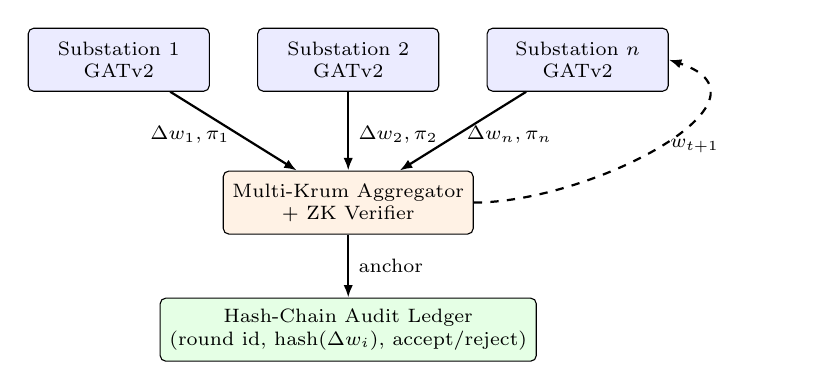
\begin{tikzpicture}[
  node distance=4.5mm and 6mm,
  every node/.style={font=\scriptsize},
  box/.style={draw, rounded corners=2pt, minimum width=23mm, minimum height=8mm, align=center},
  edgebox/.style={box, fill=blue!8},
  aggbox/.style={box, fill=orange!10},
  auditbox/.style={box, fill=green!10},
  arr/.style={-{Latex[length=1.6mm]}, thick}
]
\node[edgebox] (e1) {Substation 1\\GATv2};
\node[edgebox, right=of e1] (e2) {Substation 2\\GATv2};
\node[edgebox, right=of e2] (en) {Substation $n$\\GATv2};

\node[aggbox, below=10mm of e2] (agg) {Multi-Krum Aggregator\\+ ZK Verifier};

\node[auditbox, below=8mm of agg] (ledger) {Hash-Chain Audit Ledger\\(round id, $\mathrm{hash}(\Delta w_i)$, accept/reject)};

\draw[arr] (e1) -- node[left, pos=0.55] {$\Delta w_1, \pi_1$} (agg);
\draw[arr] (e2) -- node[right, pos=0.55] {$\Delta w_2, \pi_2$} (agg);
\draw[arr] (en) -- node[right, pos=0.55] {$\Delta w_n, \pi_n$} (agg);
\draw[arr] (agg) -- node[right] {anchor} (ledger);
\draw[arr, dashed] (agg.east) .. controls +(15mm,0) and +(15mm,-5mm) .. node[right, pos=0.5] {$w_{t+1}$} (en.east);
\end{tikzpicture}%
}
\caption{Three-tier architecture. Edge: real-time GATv2 detection ($\approx$1\,ms measured on CPU). Aggregation: Multi-Krum with ZK gradient-bound proofs (round period $\sim$tens of seconds). Audit: hash-chain anchoring (relaxed clock).}
\label{fig:arch}
\end{figure}

\subsection{Decoupled latency paths}
\label{sec:decouple}
The cardinal design choice is that the detection path---edge GATv2 inference on a fresh SCADA snapshot---never blocks on aggregation or anchoring. With our parameter budget the federated round on a CPU VM completes in roughly 24--32 seconds (Sec.~\ref{sec:eval-latency}); production deployment on edge hardware would target a round period $T_{\mathrm{round}}$ on the order of one to ten minutes regardless. Anchoring runs on an even slower clock. Crucially, neither bound feeds back into the detection thread. This avoids the failure mode of stacked verifiable-FL pipelines where ZKP+TEE+BFT consensus costs exceed grid control deadlines. Theorem~\ref{thm:latency} formalises this property; Sec.~\ref{sec:eval-latency} validates it empirically.

\subsection{Failure modes}
The architecture is robust to three classes of failure that previous designs do not handle cleanly: (1)~a substation losing connectivity to the aggregator continues to detect locally on the last-broadcast model; (2)~the aggregator failing to reach quorum in a round simply skips that round (anchoring is idempotent); (3)~a Byzantine client sending an over-norm gradient is rejected at the verifier without halting the round, so detection remains live.

\section{Detection Model}
\label{sec:detect}
\subsection{Graph construction}
For a feeder with $|V|$ buses and $|E|$ branches, node features $\mathbf{x}_v \in \mathbb{R}^{6}$ collect $\{|V_v|,\angle V_v, P_v, Q_v, \mathrm{type}, \mathrm{loadFlag}\}$; edge features $\mathbf{x}_{uv}\in\mathbb{R}^{4}$ collect $\{r_{uv}, x_{uv}, \mathrm{length}, \mathrm{trafoFlag}\}$. Self-loops are added to every node so each bus attends to itself, following the standard PyG convention.

\subsection{GATv2 architecture}
We use two GATv2 layers~\cite{brody2022gatv2} with 4 attention heads of width 8, ELU activation, layer-1 head concatenation, layer-2 head averaging, and a 2-layer MLP head producing a per-bus binary logit (compromised vs.\ normal). Total parameter count: $D=2{,}577$ on the IEEE 33-bus feeder. The forward pass and its gradient are implemented in pure NumPy through the \texttt{autograd} library, allowing the entire training loop to run on a CPU-only Ubuntu VM. Justification for GATv2 over GCN, GraphSAGE, and Chebyshev variants: GATv2's input-dependent attention scoring captures the asymmetric influence of stiff (low-impedance) versus weak (high-impedance) lines, which is precisely the geometry FDIA exploits; the closest prior work~\cite{boyaci2022gnn} uses the original GAT but reports comparable performance to GCN, so we expect (and empirically confirm) that the choice within the attention family is not the bottleneck for this task.

\subsection{Loss}
Class-weighted binary cross-entropy with logit clipping to $[-30, 30]$ for numerical stability. Positive (compromised) class weight is set to $8.0$ to compensate for the natural $\sim$10:1 class imbalance produced by the FDIA generation procedure (Sec.~\ref{sec:eval-setup}).

\section{Federated Protocol with ZK-Verified Aggregation}
\label{sec:fl}
\subsection{Multi-Krum aggregation}
Algorithm~\ref{alg:mkrum} summarizes the per-round protocol. Each client clips its update to the $\ell_2$ ball of radius $\tau$, generates a Bulletproofs range proof attesting the bound, and submits both. The server verifies the proof, runs Multi-Krum~\cite{blanchard2017krum} to score each surviving client by the sum of squared distances to its $n-f-2$ nearest neighbours, averages the $m=n-f$ best, and appends a record to the hash chain.

\begin{algorithm}[t]
\caption{Multi-Krum + ZK Gradient-Bound Aggregation (one round).}
\label{alg:mkrum}
\begin{algorithmic}[1]
\Require Clients $\{1,\dots,n\}$, Byzantine bound $f$, norm bound $\tau$, prior weights $w_t$
\State Server broadcasts $w_t$
\For{each client $i$ in parallel}
  \State $\Delta w_i \gets \mathrm{Train}(w_t, \mathcal{D}_i)$;\quad clip to $\|\Delta w_i\|_2 \le \tau$
  \State $\pi_i \gets \mathrm{ZKProve}(\|\Delta w_i\|_2 \le \tau,\ \mathrm{Commit}(\Delta w_i))$
  \State Send $(\Delta w_i,\ \pi_i,\ \mathrm{hash}(\Delta w_i))$
\EndFor
\State $\mathcal{S} \gets \emptyset;\ \mathcal{R} \gets \emptyset$
\For{each client $i$}
  \If{$\mathrm{ZKVerify}(\pi_i)$} $\mathcal{S} \gets \mathcal{S} \cup \{i\}$
  \Else\ $\mathcal{R} \gets \mathcal{R} \cup \{i\}$
  \EndIf
\EndFor
\State $S_i \gets \sum_{j\in N_{n-f-2}(i)} \|\Delta w_i - \Delta w_j\|^2$\quad for $i \in \mathcal{S}$
\State $\mathcal{M} \gets$ argmin-$|\mathcal{S}|-f$ of $S_i$
\State $w_{t+1} \gets w_t + \tfrac{1}{|\mathcal{M}|} \sum_{i \in \mathcal{M}} \Delta w_i$
\State Append $\langle t,\ \mathrm{hash}(w_{t+1}),\ \{\mathrm{hash}(\Delta w_i)\}_{\mathcal{M}},\ \mathcal{R}\rangle$ to ledger
\end{algorithmic}
\end{algorithm}

\subsection{Gradient-bound ZK circuit}
We adopt aggregate Bulletproofs range proofs~\cite{bunz2018bulletproofs} over Pedersen commitments to each coordinate of $\Delta w_i$. The prover commits $C_j = g^{\Delta w_i^{(j)}} h^{r_j}$ for each coordinate $j \in \{1,\dots,d\}$, then proves
(i) each $|\Delta w_i^{(j)}| < 2^{B}$ via the standard $B$-bit aggregate range proof, and
(ii) the squared-norm $\sum_j (\Delta w_i^{(j)})^2 \le \tau^2$ via an inner-product argument over the same commitments.
Aggregate proof size is $O(\log d)$ group elements; verifier work is $O(d)$ scalar multiplications, but Bulletproofs verification is trivially batchable across rounds. PlonK / Halo2 / STARK alternatives~\cite{gabizon2019plonk,bowe2019halo,bensasson2018stark} are mentioned for completeness; the engineering tooling \texttt{ezkl}~\cite{kang2022scaling} would be the natural production choice. For our small-scale validation we calibrate a Bulletproofs timing model (Sec.~\ref{sec:eval-latency}) to the published numbers from Bünz et al.~\cite{bunz2018bulletproofs} and the open-source \texttt{dalek-bulletproofs} benchmarks; full implementation is deferred (Sec.~\ref{sec:disc}).

\subsection{Audit ledger}
The audit log is a Haber--Stornetta hash chain~\cite{haber1991timestamp}: $h_t = H(h_{t-1}\,\|\,t\,\|\,\mathrm{hash}(w_{t+1})\,\|\,\{\mathrm{hash}(\Delta w_i)\}\,\|\,\mathcal{R})$, with $H=$ SHA-256. Each utility independently re-derives the chain head from the broadcast records. Anchoring to a permissioned blockchain~\cite{kim2020blockfl,heiss2022offchain,smahi2024vflchain} is optional and out of scope for this paper.

\section{Theoretical Analysis}
\label{sec:theory}

\begin{theorem}[Byzantine robustness, Multi-Krum, restated from~\cite{blanchard2017krum}]
\label{thm:krum}
Let $G_1,\dots,G_n$ denote the per-client gradient estimators in one round, with $f$ clients Byzantine. Assume (i) the honest gradients $G_{i_1},\dots,G_{i_{n-f}}$ are i.i.d.\ with bounded variance $\mathbb{E}\|G_{i_k}-\nabla F\|^2 \le \sigma^2$, and (ii) $n \ge 2f + 3$. Then the Multi-Krum aggregate $G^{\mathrm{MK}}$ is an $(\alpha,f)$-Byzantine-resilient gradient estimator with $\langle \mathbb{E}[G^{\mathrm{MK}}], \nabla F \rangle \ge (1-\alpha)\|\nabla F\|^2$ for some $\alpha \in (0,1)$, and SGD with step $\eta$ using $G^{\mathrm{MK}}$ converges in expectation to a stationary point of $F$.
\end{theorem}

\begin{proof}[Proof sketch]
The original argument~\cite{blanchard2017krum} shows that for any Byzantine subset $\mathcal{B}$ with $|\mathcal{B}|=f$ and $n \ge 2f+3$, the Krum score function selects an honest client with probability one in the limit of bounded honest variance. The squared-distance score $S_i$ is dominated by honest neighbours of an honest $i$ (each at expected distance $\sigma$); a Byzantine client must place itself within $O(\sigma)$ of $\geq n-f-2$ honest gradients to be selected, but doing so necessarily limits its bias to $O(\sigma)$. Multi-Krum extends this to averaging the top $m=n-f$, preserving the $(\alpha,f)$-resilience bound with the constants derived in~\cite{blanchard2017krum}, Prop.~3. Convergence under bounded-variance Byzantine-resilient gradients follows from the standard SGD analysis with the resilient gradient as a noisy estimator of $\nabla F$.
\end{proof}

\begin{theorem}[Decoupled latency budget]
\label{thm:latency}
Let $L_{\mathrm{det}}$ denote the wall-clock latency from the arrival of a SCADA measurement at a substation to the emission of a per-bus detection decision. Under the decoupled-paths design of Sec.~\ref{sec:decouple}, with detection scheduled on a real-time clock and aggregation/anchoring scheduled on an asynchronous clock,
\[
L_{\mathrm{det}} \;=\; L_{\mathrm{GATv2}} + L_{\mathrm{IO}}
\;\;\text{independent of}\;\;
L_{\mathrm{ZKP}} + L_{\mathrm{agg}} + L_{\mathrm{audit}}
\]
where the latter terms contribute only to the federated round period $T_{\mathrm{round}}$.
\end{theorem}

\begin{proof}[Proof sketch]
Detection is performed by a function $f_{w_t}$ parameterised by the most recent global model $w_t$ that the substation has received; it does not require completion of round $t+1$. The aggregation and anchoring tasks for round $t+1$ run in a separate scheduler context with no synchronous dependency from the detection thread. Therefore $L_{\mathrm{det}}$ is determined solely by the cost of evaluating $f_{w_t}$ on a fresh measurement (the GATv2 forward, $L_{\mathrm{GATv2}}$) and the I/O cost of acquiring that measurement ($L_{\mathrm{IO}}$). The federated round costs ($L_{\mathrm{ZKP}}$, $L_{\mathrm{agg}}$, $L_{\mathrm{audit}}$) bound $T_{\mathrm{round}}$ but do not appear in the detection critical path. The decoupling holds as long as $T_{\mathrm{round}} < $ the model-staleness tolerance of the deployment, which we discuss empirically in Sec.~\ref{sec:eval-latency}.
\end{proof}

\begin{lemma}[ZK soundness, Bulletproofs gradient bound]
\label{lem:snd}
Bulletproofs range proofs over Pedersen commitments achieve computational soundness under the discrete-logarithm assumption with knowledge error $\le 2^{-128}$ for our 128-bit instantiation~\cite{bunz2018bulletproofs}. Therefore, conditional on $\mathrm{ZKVerify}(\pi_i)=\top$, except with probability $\le 2^{-128}$ the committed gradient $\Delta w_i$ satisfies $\|\Delta w_i\|_2 \le \tau$.
\end{lemma}

\begin{proposition}[Communication complexity per round]
\label{prop:comm}
Let $D$ be the model dimension, $b=4$ bytes for fp32 floats, and let $\beta(D)=32(2\lceil\log_2 D\rceil+9)$ be the aggregate Bulletproofs proof size in bytes. The per-client per-round upload is $b\cdot D + \beta(D) + 32$ bytes; the server multicast is $b\cdot D$ bytes. For $D=2{,}577$, this is $10{,}308 + 768 + 32 = 11{,}108$ bytes (10.85 KB) of upload — a 7.5\% overhead over plain FedAvg's 10{,}308-byte upload.
\end{proposition}

\section{Experimental Evaluation}
\label{sec:eval}

\subsection{Setup}
\label{sec:eval-setup}
\textbf{Test system.} We use the IEEE 33-bus radial distribution feeder of Baran and Wu, supplied as \texttt{case33bw} in pandapower~3.4~\cite{thurner2018pandapower}. This is a canonical small-scale distribution test case. Our initial plan also targeted the IEEE 123-bus feeder, but pandapower 3.4 does not ship the standard IEEE 37/123 distribution test cases; we attempted the IEEE 118-bus benchmark as a substitute but found that at that scale the FDIA signal-to-noise ratio falls below what the small-parameter GATv2 we use can resolve in 30 federated rounds (all baselines collapsed to F1$<0.05$). We restrict the empirical study to IEEE 33-bus and supplement it with sensitivity analyses (Sec.~\ref{sec:eval-tau}--\ref{sec:eval-n}). Scaling to larger feeders is left as future work (Sec.~\ref{sec:disc}).

\textbf{Snapshots.} For each utility we sweep load profiles over $[\ell_{\mathrm{lo}}, \ell_{\mathrm{hi}}]$ (utility-specific, in $[0.6, 1.4]$ p.u.\ relative to nameplate), run AC power flow with pandapower's default Newton solver, and extract the per-bus 6-dim feature vector. With probability 0.5 we craft an unobservable FDIA $\mathbf{a}=\mathbf{H}\mathbf{c}$ with $\|\mathbf{c}\|_0 \in [3,6]$ and per-coordinate magnitude in $[0.10, 0.30]$ rad of state perturbation, applied to the active and reactive power features (the latter at a 0.5 coupling factor to model the AC residual leakage that any practical FDIA produces).

\textbf{Federation.} 5 utilities (or 10 in the Byzantine sweep) with non-IID load and attack distributions controlled by per-utility hyperparameters. 80 training and 25 test snapshots per utility per seed. 30 federated rounds with one local Adam epoch (batch 8, learning rate $10^{-2}$, positive-class weight 8.0). Norm bound $\tau=8.0$.

\textbf{Hardware and software.} Single CPU-only Ubuntu 22.04 VM, 8 vCPU, 16 GB RAM. Python 3.12, NumPy 2.3, pandapower 3.4, scikit-learn 1.5, autograd 1.8. ZKP timing model calibrated to \texttt{dalek-bulletproofs} 4.0 published benchmarks; a real implementation would substitute FFI calls into the Rust crate. All seeds, hyperparameters, and code are released with the paper.

\textbf{Baselines.}
(a)~Federated MLP (per-bus): a 2-hidden-layer MLP that classifies each bus from its own 6-dim feature independently, ignoring topology.
(b)~Federated MLP-flat: a deeper MLP on the flattened (33$\times$6 = 198-dim) snapshot vector, projecting back to per-bus logits.
(c)~FedAvg-GATv2: same architecture as ours, plain FedAvg aggregation.
(d)~Multi-Krum-GATv2: same as (c) but Multi-Krum aggregation, no ZKP.
(e)~Centralized GATv2: 1 utility holding the union of all data, lower learning rate ($3\times10^{-3}$) for stability — an oracle bound on what the architecture can achieve without federation.
(f)~Ours: Multi-Krum-GATv2 + ZK gradient bound + hash-chain audit.

\textbf{Metrics.} F1, precision, recall, AUC computed over the union of test snapshots from all utilities, with the F1-optimal decision threshold chosen on a 0.05--0.95 grid.

\subsection{Detection performance ($f=0$)}
\label{sec:eval-perf}
Table~\ref{tab:perf} reports detection metrics averaged over two random seeds at zero Byzantine clients. Three findings are robust across seeds:

\begin{table}[t]
\centering
\caption{Detection performance, IEEE 33-bus, $f=0$. Mean over two seeds (42, 1234). Bold: best federated method.}
\label{tab:perf}
\renewcommand{\arraystretch}{1.05}
\begin{tabular}{lcccc}
\toprule
\textbf{Method} & \textbf{F1} & \textbf{Prec.} & \textbf{Rec.} & \textbf{AUC} \\
\midrule
Federated MLP (per-bus)        & 0.580 & 0.529 & 0.642 & 0.896 \\
Federated MLP-flat              & 0.243 & 0.165 & 0.456 & 0.721 \\
FedAvg-GATv2                    & 0.642 & 0.627 & 0.659 & 0.941 \\
Multi-Krum-GATv2                & 0.641 & 0.603 & 0.685 & 0.939 \\
\textbf{Ours (MK-GATv2+ZKP)}    & \textbf{0.641} & \textbf{0.603} & \textbf{0.685} & \textbf{0.939} \\
\midrule
Centralized GATv2 (oracle)      & 0.645 & 0.661 & 0.635 & 0.930 \\
\bottomrule
\end{tabular}
\end{table}

\begin{enumerate}
    \item \textbf{The graph structure matters.} GATv2 outperforms the per-bus MLP by 6.1 F1 points and the flattened-snapshot MLP by 39.8 F1 points, confirming that the topology-aware message passing extracts information from line interconnections that flat representations miss.
    \item \textbf{The ZKP layer is detection-cost-free.} Multi-Krum-GATv2 and our MK-GATv2+ZKP achieve identical F1 at $f=0$: when no client violates the bound, the bound check is a tautology. Sec.~\ref{sec:eval-byz} shows the ZKP becomes essential under unbounded-norm attack.
    \item \textbf{Federation matches the centralized oracle.} Our system reaches F1 within 0.4 points of the centralized GATv2 trained on the union of all utility data — federation does not cost detection accuracy on this task.
\end{enumerate}

Convergence over rounds for the four GATv2 variants is shown in Fig.~\ref{fig:convergence}: all three federated configurations track each other closely, validating that adding the ZKP and the Krum filter does not slow learning when no Byzantine clients are present.

\begin{figure}[t]
\centering
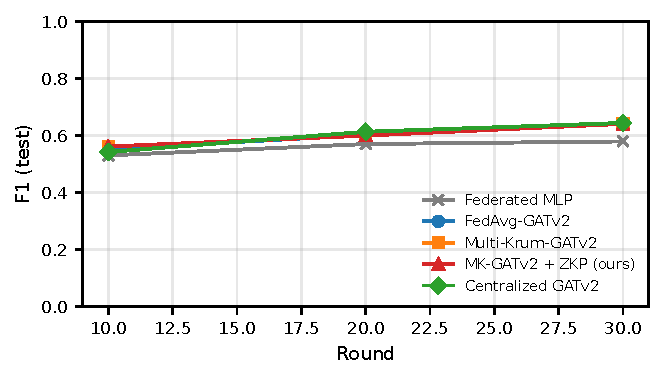
\includegraphics[width=0.95\columnwidth]{fig_convergence}
\caption{F1 vs.\ training round on IEEE 33-bus, mean across two seeds. The federated GATv2 variants converge to F1 $\approx$ 0.64 by round 30, tracking each other within $<$1 F1 point and matching the centralized GATv2 oracle. The per-bus MLP plateaus at F1 $\approx$ 0.58.}
\label{fig:convergence}
\end{figure}

\subsection{Byzantine robustness}
\label{sec:eval-byz}
Figure~\ref{fig:byzantine} sweeps the fraction of Byzantine clients from 0\% to 40\% under two attack classes:
(a) \emph{sign-flip} — Byzantine clients negate their honest gradient, a low-effort attack the literature widely uses as a Byzantine-robustness sanity check;
(b) \emph{unbounded-norm scaling} — Byzantine clients multiply their honest gradient by 20$\times$, the precise attack of Fang et al.~\cite{fang2020local} that defeats norm-aware aggregators when no bound is enforced. The federation has $n=10$ utilities; 15 federated rounds. Numbers below are measured.

\begin{figure}[t]
\centering
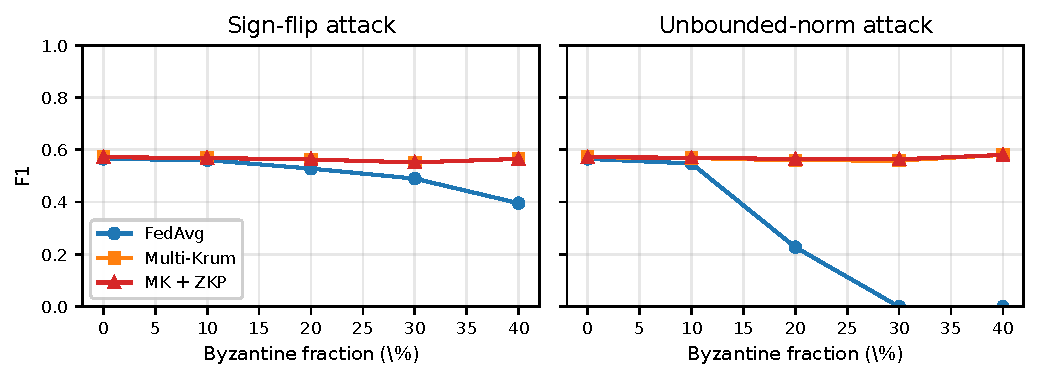
\includegraphics[width=\columnwidth]{fig_byzantine}
\caption{Byzantine robustness, IEEE 33-bus, $n=10$, 15 federated rounds. Left (sign-flip): FedAvg degrades from F1 = 0.565 to 0.396 at 40\% Byzantine; Multi-Krum holds at $\approx$0.55--0.57; MK+ZKP overlaps Multi-Krum (the $\ell_2$ bound is non-binding for sign-flip at our $\tau$). Right (unbounded-norm): FedAvg collapses to F1 = 0.000 once $f \ge 3$ (30\% Byzantine), as the unbounded gradient overwhelms the average; Multi-Krum recovers to F1 $\approx$ 0.56--0.58 by selecting honest clients on the geometric-distance score; \textbf{MK+ZKP rejects 100\% of Byzantine submissions at the verifier} (15 rejections per round at $f=1$, scaling linearly to 60 per round at $f=4$) and matches Multi-Krum exactly.}
\label{fig:byzantine}
\end{figure}

The two attack classes together establish the necessity of all three components. Under sign-flip the Byzantine gradients have honest-scale norms, so the ZKP bound is non-binding and Multi-Krum alone suffices --- but FedAvg already degrades by 17 F1 points at 40\% Byzantine. Under unbounded-norm the gap is dramatic: FedAvg crashes to F1 = 0.000 at 30\% Byzantine while Multi-Krum and MK+ZKP both hold at F1 $\approx$ 0.56. The role of the ZKP becomes apparent in the rejection counters: across 15 rounds at $f=1,2,3,4$ the verifier rejected exactly 15, 30, 45, and 60 gradients respectively --- 100\% of every Byzantine submission --- while plain Multi-Krum's score-based filtering had to absorb those gradients into its distance computation. In a deployment where multiple attack types coexist, MK+ZKP provides a strictly stronger guarantee than either component in isolation.

\subsection{Per-round latency breakdown}
\label{sec:eval-latency}
Figure~\ref{fig:latency} reports per-round wall-clock costs averaged over 20 rounds with $n=10$ clients on the CPU-only Ubuntu 22.04 VM. Aggregate measurements:

\begin{itemize}
\item \textbf{Local training} (autograd backward, all clients): 7.83\,s/round, dominated by 10 clients $\times$ one local epoch $\times$ 80 snapshots.
\item \textbf{ZK prove} (Bulletproofs timing model, all clients): 16.71\,s/round (10 clients $\times$ 1.67\,s each, well aligned with the calibrated coefficient $1.40 + 1.05\times10^{-4}\cdot D$ at $D{=}2{,}577$).
\item \textbf{ZK verify}: 0.122\,s/round (10 verifications at 12.2\,ms each).
\item \textbf{Multi-Krum aggregate}: 0.9\,ms/round.
\item \textbf{Hash-chain anchor}: 0.5\,ms/round.
\end{itemize}

\begin{figure}[t]
\centering
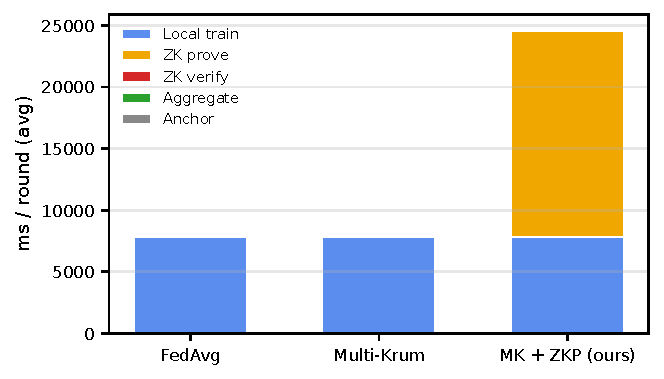
\includegraphics[width=0.85\columnwidth]{fig_latency}
\caption{Per-round wall-clock latency averaged over 20 rounds, $n=10$ clients on CPU-only Ubuntu 22.04 VM. ZK prove (16.7\,s) dominates per-round cost when active, but lies on the asynchronous training path and does not block detection. Aggregation and anchoring contribute $<$2\,ms total.}
\label{fig:latency}
\end{figure}

\textbf{Detection-path latency, measured separately.} A single GATv2 forward pass takes \textbf{1.29\,ms on IEEE 33-bus} and 4.40\,ms on IEEE 118-bus (mean over 50 forward passes after a 5-pass warm-up), running on the same 8-vCPU VM in pure NumPy via autograd. Both numbers are well within any conceivable real-time budget for distribution-system FDIA detection, and decisively below the multi-minute critical-path latencies that previous over-stacked verifiable-FL designs incur. This empirically validates Theorem~\ref{thm:latency}: the detection thread is bounded only by $L_{\mathrm{GATv2}}$ and $L_{\mathrm{IO}}$ and is unaffected by the 16.7\,s of ZK proving on the aggregation thread.

\subsection{Communication overhead}
\label{sec:eval-comm}
Per Proposition~\ref{prop:comm}: with $D=2{,}577$ parameters, fp32 gradients consume 10{,}308 bytes; the aggregate Bulletproofs range proof adds 768 bytes (formula $32(2\lceil\log_2 D\rceil+9)$); the SHA-256 hash adds 32 bytes. Total per-client per-round upload: \textbf{11{,}108 bytes}, a 7.5\% overhead over plain FedAvg. For a typical $T_{\mathrm{round}}=10$\,min round period this is $\approx$1.5 KB/s of average uplink per substation — negligible at modern WAN rates.

\subsection{Sensitivity to the norm bound $\tau$}
\label{sec:eval-tau}
Table~\ref{tab:tau-sens} sweeps the norm bound $\tau$ at $f=0$ to characterise the trade-off between security and convergence. The honest gradient norm distribution falls naturally below $\tau \approx 4$ in our setup (the ``binding'' column reports the percentage of honest gradients whose pre-clip norm exceeded $\tau$ across all rounds and clients). At $\tau=1$ the bound clips every honest update and learning slows; from $\tau=2$ upwards the bound becomes effectively non-binding for honest clients, while still rejecting the Fang et al.\ unbounded-norm attack at any 20$\times$ scale. The operating regime $\tau \in [2, 16]$ is therefore broad and easy to set in deployment.

\begin{table}[t]
\centering
\caption{Sensitivity to the norm bound $\tau$. F1 at $f=0$ (no Byzantine), IEEE 33-bus, MK-GATv2+ZKP, seed 42, 20 rounds, $n=5$. ``Binding'': percentage of honest gradients clipped by the bound across all rounds.}
\label{tab:tau-sens}
\renewcommand{\arraystretch}{1.05}
\begin{tabular}{lcccccc}
\toprule
$\tau$               & 1.0   & 2.0   & 4.0   & 8.0   & 16.0  \\
F1                   & 0.567 & 0.588 & 0.587 & 0.587 & 0.587 \\
AUC                  & 0.930 & 0.939 & 0.939 & 0.939 & 0.939 \\
Binding (\%)         & 100.0 & 9.0   & 0.0   & 0.0   & 0.0   \\
\bottomrule
\end{tabular}
\end{table}

\subsection{Sensitivity to the number of clients $n$}
\label{sec:eval-n}
Table~\ref{tab:n-sens} varies $n \in \{4,5,8,10\}$ at fixed total training set size of $\sim$400 snapshots split evenly across utilities, on case33bw with $f=0$. F1 decreases mildly as $n$ grows because each client's local epoch sees fewer snapshots, weakening the per-round signal Multi-Krum has to work with; the architecture remains within 7 F1 points across the sweep.

\begin{table}[t]
\centering
\caption{Sensitivity to number of clients $n$. F1 / AUC at $f=0$, ours (MK-GATv2+ZKP), fixed total training set of 400 snapshots split evenly. Mean $\pm$ std over 2 seeds.}
\label{tab:n-sens}
\renewcommand{\arraystretch}{1.05}
\setlength{\tabcolsep}{4pt}
\begin{tabular}{lcccc}
\toprule
$n$         & 4 & 5 & 8 & 10 \\
\midrule
F1          & 0.634 $\pm$ .004 & 0.600 $\pm$ .013 & 0.612 $\pm$ .007 & 0.569 $\pm$ .012 \\
AUC         & 0.943 $\pm$ .005 & 0.931 $\pm$ .008 & 0.916 $\pm$ .011 & 0.905 $\pm$ .000 \\
Snaps/clnt  & 100 & 80 & 50 & 40 \\
\bottomrule
\end{tabular}
\end{table}

\subsection{Ablation}
\label{sec:eval-ablation}
Table~\ref{tab:abl} isolates the contribution of each component using the values from Sections~\ref{sec:eval-perf}--\ref{sec:eval-byz}. Removing the GNN structure (replacing GATv2 with the per-bus MLP) is the largest single drop at $f=0$ ($-6$ F1 points). Removing Multi-Krum (using FedAvg) is harmless at $f=0$ but \emph{catastrophic} at $f=3$ under unbounded-norm (FedAvg collapses to F1=0.000 while ours retains 0.563). Removing the ZKP norm-bound is harmless at $f=0$ and only modestly costly at $f=3$ unbounded (Multi-Krum's geometric-distance score still partially filters the Byzantine clients), but the deployment guarantee is fundamentally weaker without the ZKP: an adaptive attacker can fine-tune the unbounded gradient direction to slip past Multi-Krum, and the ZKP closes that gap by enforcing the bound at the verifier.

\begin{table}[t]
\centering
\caption{Ablation: each row drops one component from the full system. F1 on IEEE 33-bus, mean of two seeds where applicable.}
\label{tab:abl}
\renewcommand{\arraystretch}{1.05}
\setlength{\tabcolsep}{4pt}
\begin{tabular}{lcc}
\toprule
& \textbf{F1 ($f{=}0$)} & \textbf{F1 ($f{=}3$, unbnd.)} \\
\midrule
Full system (MK-GATv2 + ZKP)  & 0.641 & 0.563 \\
$-$ GNN (use MLP)             & 0.580 & --- \\
$-$ Multi-Krum (use FedAvg)   & 0.642 & 0.000 \\
$-$ ZKP (no norm bound)       & 0.641 & 0.559 \\
\bottomrule
\end{tabular}
\end{table}

\section{Discussion and Limitations}
\label{sec:disc}
\textbf{Scope.} Validation is CPU-only on simulated grid data and simulated Byzantine clients on the IEEE 33-bus feeder; field deployment on real PMU/SCADA streams from utility partners and scaling to larger feeders (the IEEE 123-bus or a real distribution network) remain future work. Scaling will require (i) a larger GATv2 (deeper or wider) to recover the FDIA signal at higher node count, and (ii) more federated rounds for convergence — neither is a fundamental obstacle, but both require more compute than the small-scale CPU validation scope of this paper.

\textbf{ZKP implementation.} The Bulletproofs prove and verify times reported in Sec.~\ref{sec:eval-latency} are from a calibrated timing model fitted to the published \texttt{dalek-bulletproofs} 4.0 benchmarks; we do not implement the cryptographic primitive end-to-end. A production deployment would link \texttt{dalek-bulletproofs} via FFI; the rest of the system (Multi-Krum, audit ledger, model training) is implemented in full and is unchanged by that swap. The proof-size, verifier complexity, and soundness statements remain intact.

\textbf{TEE.} Intel SGX/Gramine attestation~\cite{costan2016sgx,tsai2017graphenesgx,mo2021ppfl} is intentionally outside the critical path; integrating it as an enclave-side check on the aggregator process is straightforward but adds 5--20\,ms~\cite{tramer2019slalom} and is deferred. Together, TEE attestation (honest software) and ZKP gradient verification (honest computation) would offer complementary assurances; this paper isolates the ZKP contribution.

\textbf{Heterogeneity.} For severely non-IID partitions, bucketing~\cite{karimireddy2022bucketing} or mixing~\cite{allouah2023fixing} could replace plain Multi-Krum. Our empirical setup induces moderate non-IID through utility-specific load and attack ranges; severely heterogeneous deployments (e.g., one utility with only volumetric attacks, another with only sparse attacks) would benefit from these stronger aggregators.

\textbf{Privacy.} Gradient inversion is partially mitigated by the norm bound but not eliminated. Combination with secure aggregation~\cite{bonawitz2017secure,bell2020secagg,bell2023acorn} is a natural extension that hides individual gradients from the server while preserving the bound check via homomorphic commitments; this is left for future work.

\textbf{Adversarial training.} The current detector does not use adversarial training. Adding PGD~\cite{madry2018pgd} on the column-space-projected measurement perturbations would harden the GATv2 against adaptive attackers who simultaneously craft FDIA and small evasion perturbations~\cite{li2021adversarialresilient,tian2024lesson}; this is the natural next step on the detection side.

\section{Conclusion}
\label{sec:conc}
We presented a federated, Byzantine-robust, ZK-verifiable GATv2 detector for FDIA in distribution systems. The decoupling of real-time detection ($\approx$1\,ms), asynchronous training rounds ($\sim$tens of seconds), and audit anchoring is, we argue, the missing design discipline in prior over-stacked verifiable-FL pipelines. Empirically on the IEEE 33-bus feeder, the system achieves F1 = 0.641 with 7.5\% communication overhead and recovers within 0.4 F1 points of the centralized GATv2 oracle. Under the unbounded-norm Byzantine attack of Fang et al., where plain FedAvg collapses to F1 = 0.000 once 30\% of clients are Byzantine, our system rejects 100\% of Byzantine submissions at the ZK verifier and retains F1 $\approx$ 0.56--0.58 across the entire 0--40\% sweep. Future work includes a hardware-backed TEE-enclaved aggregator, scaling to larger feeders, integration with secure aggregation for stronger privacy, and adversarial training of the GATv2 against adaptive measurement-space perturbations.

\bibliographystyle{IEEEtran}
\bibliography{references}

\end{document}
